\documentclass{scrartcl}
\usepackage{amsmath, amssymb, amsfonts, amsthm, graphicx}
\usepackage[sexy]{evan}

\usepackage{setspace}
\setstretch{1.1}

\begin{document}

\begin{titlepage}
   \begin{center}
       \vspace*{1.5cm}
       \huge \textbf{Inversion!}

       \vspace{0.5cm}
       \Large \textbf{Tired of annoying circles? There's a method called Inverting and Cheesing the heck out of it.}
            
       \vspace{1.5cm}

       \textbf{Brian and Celestia}

       \vfill
            
        
\includegraphics[scale=0.2]{mizuki.jpg}
    \end{center}    
\end{titlepage}
\newpage
\title{Inversion!}
\author{Brian and Celestia}

\section{Introduction}
A lot of issues in geometry problems come from dealing with annoying circles, especially when they intersect and you cannot angle chase your way out of it. Length chasing doesn't always work either because they are circles... except we don't have to allow them to stay as circles.

Before we get into what inversion is, we should go over how its definition was motivated first. Take a look at the following diagram:
\begin{center}
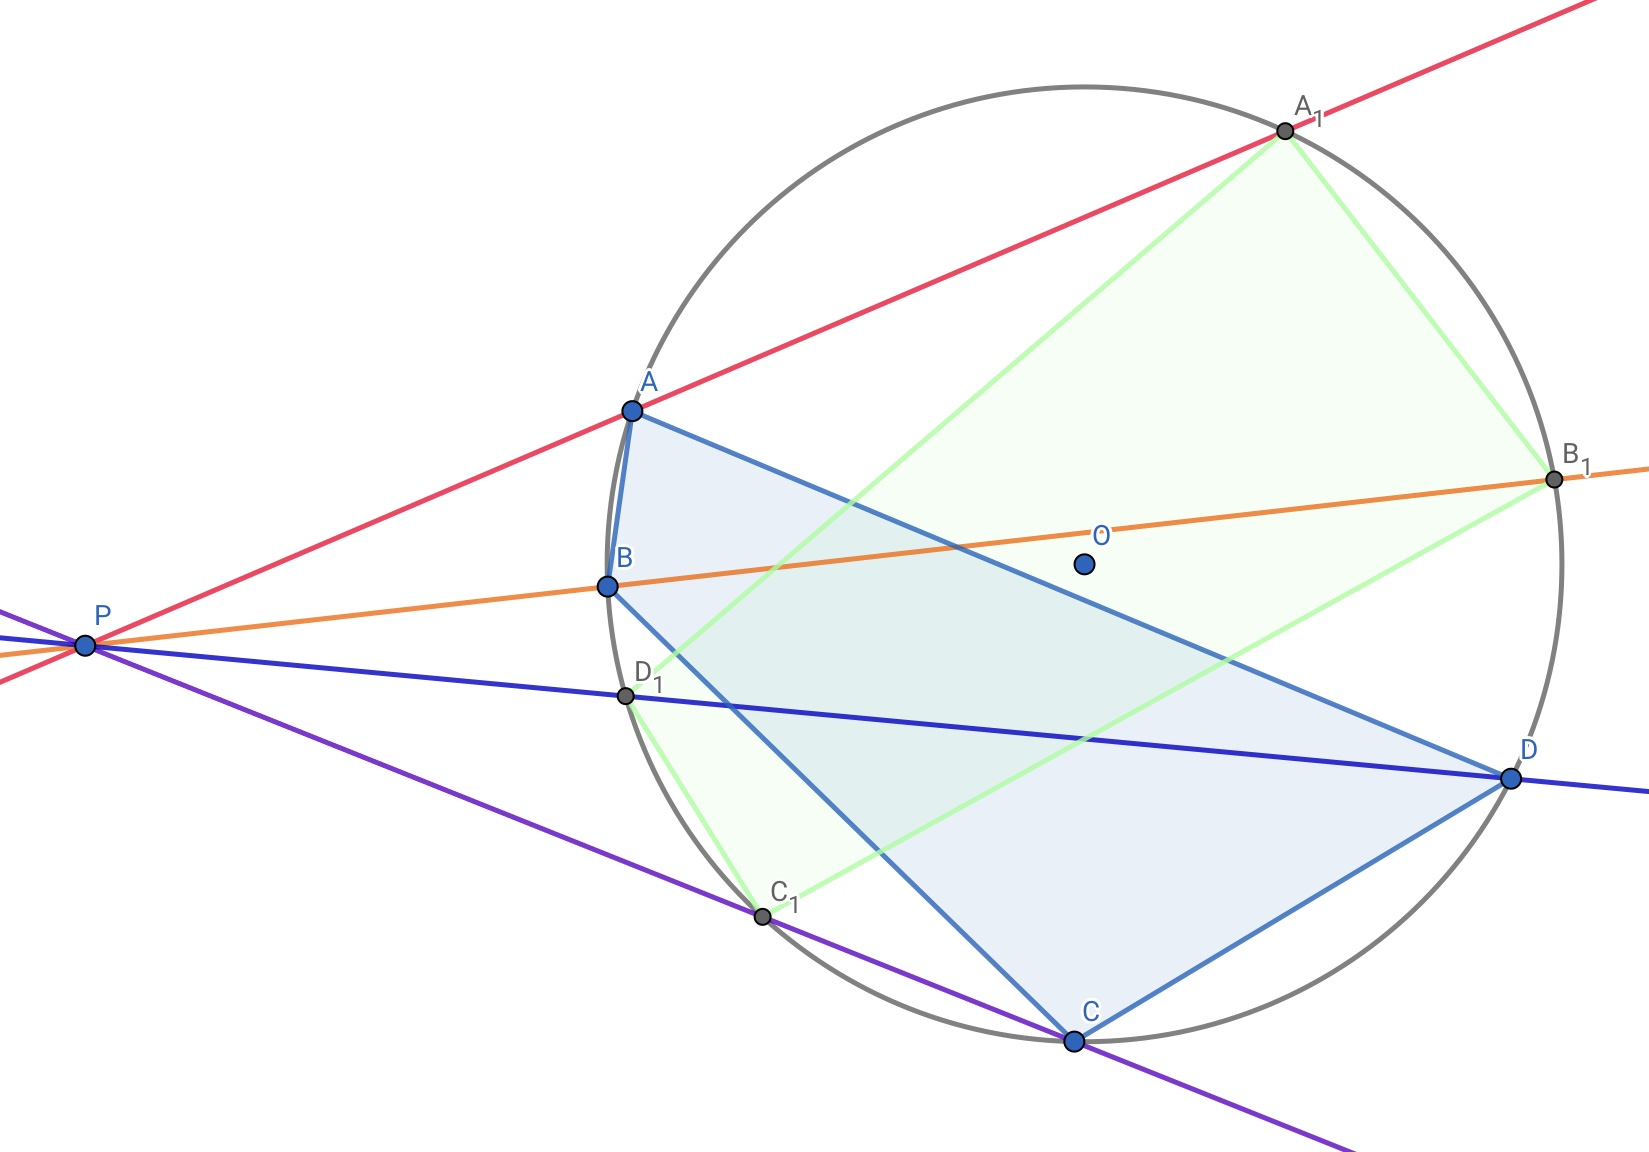
\includegraphics[scale=0.2]{pop.jpeg}
\end{center}
Observe that $PA \cdot PA_1 = PB \cdot PB_1 = PC \cdot PC_1 = PD \cdot PD_1$ , and the quadrilateral $A_1 B_1 C_1 D_1$ is cyclic as well, so if we let $r$ be the power of $P$ with respect to this circle, then the transformation sending a point $Q$ to another point $Q'$ on the line $PQ$ such that the directed length product $PQ \cdot PQ' = r$ will preserve this entire circle. But wait, if we change $r$ then the image of the transformation just gets magnified with $P$ as a center, so no matter what $r$ is this transformation will preserve every circle not passing through it! \newline \newline
\textbf{Definition:} An $inversion$ centered at $P$ with power $r$ is the transformation sending a point $Q$ to another point $Q'$ on the line $PQ$ such that the directed length product $PQ \cdot PQ' = r$. \newline
\begin{theorem}
An inversion centered at a point $P$ will send a circle passing through $P$ to a line not passing through $P$ parallel to the tangent line to that circle at $P$. 
\end{theorem}
The proof is left to the reader as an exercise.
\begin{theorem}
(Dual of the previous one) An inversion centered at a point $P$ will send a line not passing through $P$ to a circle through $P$ such that the tangent line to it at $P$ is parallel to the initial line.
\end{theorem}
The thing that makes this so strong is that we sometimes encounter wacky circles that somehow contain important points. Inverting about one of these important points will turn it into a line that is sometimes much easier to deal with. Here is an example. \newline
\begin{problem} A triangle $ABC$ has an incenter $I$ and a variable point $D$ on the minor arc $AB$ on $(ABC)$. Define $E$ as the unique point on the segment $BC$ such that $\angle IEC = \angle ADI$. Prove that $DE$ always passes through a fixed point.
\end{problem}
\textbf{Solution:} Let $D_1$ be the intersection of $DI$ and $(ABC)$, and let $S$ be the midpoint of the minor arc $BC$. Furthermore, let $F = SD_1 \cap BC$. The motivation of these constructions is that we want to turn these angle conditions into a cyclic condition with a cyclic quadrilateral involving $I$ so that things become more manageable (note that there is another cyclic quad to be made but it isn't as nice because $I$ serves as the intersection of diagonals, not a vertex.) Observe that $\angle ISF = \angle ASD_1 = \angle ADI = \angle IEF$ therefore the quadrilateral $IESF$ is cyclic. At this point it is rather clear that $S$ should be our desired fixed point, but here comes the issue in proving it - $\angle IFE$ cannot be chased. Furthermore, what even is the significance of $F$ being the intersection of $SD_1$ and $BC?$ \newline
\begin{center}
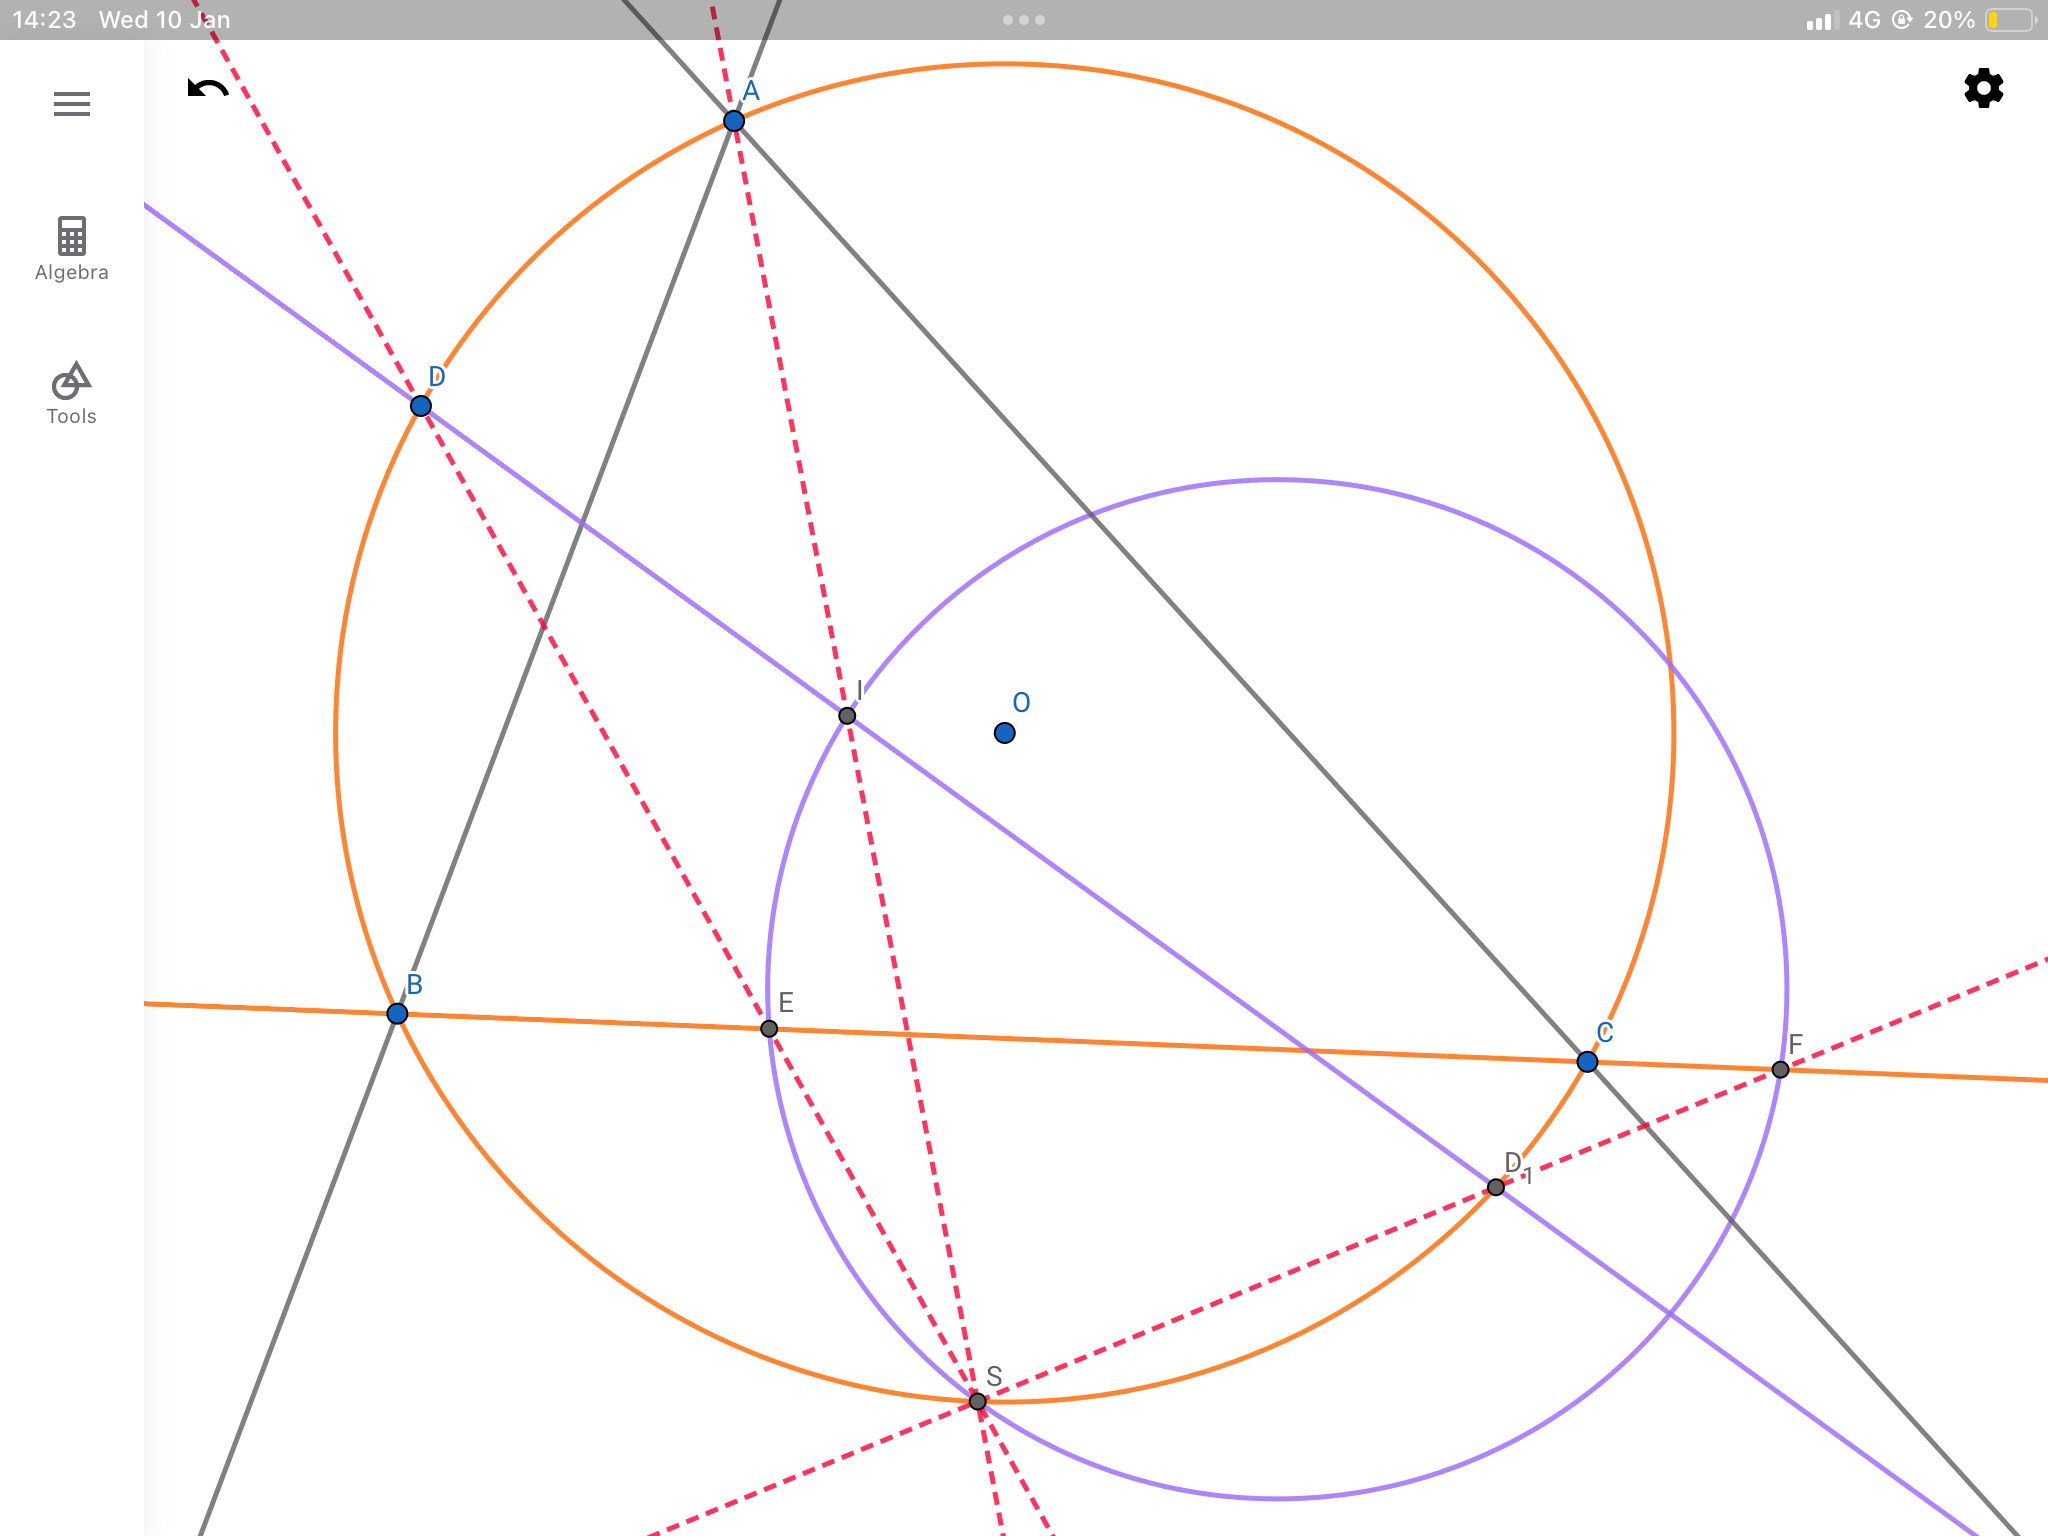
\includegraphics[scale=0.2]{IMG_4842.png}
\end{center}

\textbf{We perform an inversion centered at $S$ with power $(SI)^2$.} Since $(ABC)$ must go to a line and $I,B,C$ must stay at the same position under the inversion due to $SI = SB = SC$, we know that $(ABC)$ gets inverted to the line $BC$. Now we just need to prove that $D$ gets sent to $E$ or vice versa, but since $F$ goes to $D_1$ and $IESF$ is cyclic, this inversion sends $(IESF)$ to the line $ID_1$ and thus sends $E$ to the point on $(ABC)$ that's also on $ID_1$, which is $D$. Therefore, this inversion sends $E$ to $D$ and so $S,D,E$ are always collinear. $\square$\newline

One thing to note is that angle conditions under inversion stay relatively clean due to the fact that if $A$ is the center of inversion and it sends $P,Q$ to $P',Q'$ then from $PQQ'P'$ being cyclic we know that $\triangle APQ, \triangle AQ'P'$ are similar but with a different orientation of angles. Therefore, $\angle APQ = \angle AQ'P'$ and $AP/AQ = AQ'/AP'$.

\section{Length Chase}
Why lecture when you can just play a Numberphile video. \newline
\href{https://www.youtube.com/watch?v=bJOuzqu3MUQ&t=1268s}{https://www.youtube.com/watch?v=bJOuzqu3MUQ\&t=1268s}

\section{Meme Techniques}
\begin{problem} [EGMO 2013/5]
Let $\Omega$ be the circumcircle of triangle $ABC$. The circle $\omega$ is tangent to the sides $AC$ and $BC$, and it's internally tangent to $\Omega$ at $P$. A line parallel to AB and intersecting the interior of triangle $ABC$ is tangent to $w$ at $Q$. Prove that $\angle ACP = \angle QCB$.
\end{problem}
\textbf{Solution:} Wow, mixtilinear incircles and isogonals, this questions is begging for root bc inversion. \newline
Root bc inversion is a reflection in the A-angle bisector, followed by an inversion centered at A with power $bc$, where $b$ and $c$ are the lengths of $AC$ and $AB$. It has the following powerful properties:
\begin{itemize}
  \item $B \rightarrow C$; $C \rightarrow B$.
  \item $(ABC) \rightarrow BC$.
  \item $A$-isogonals are mapped onto each other. 
\end{itemize}
For this question, we just need to swap the letters around and invert about $C$ instead. $\Omega$ goes to $AB$, $AC$ goes to $BC$, $BC$ goes to $AC$, so $\omega$ goes to...\newline
\begin{center}
    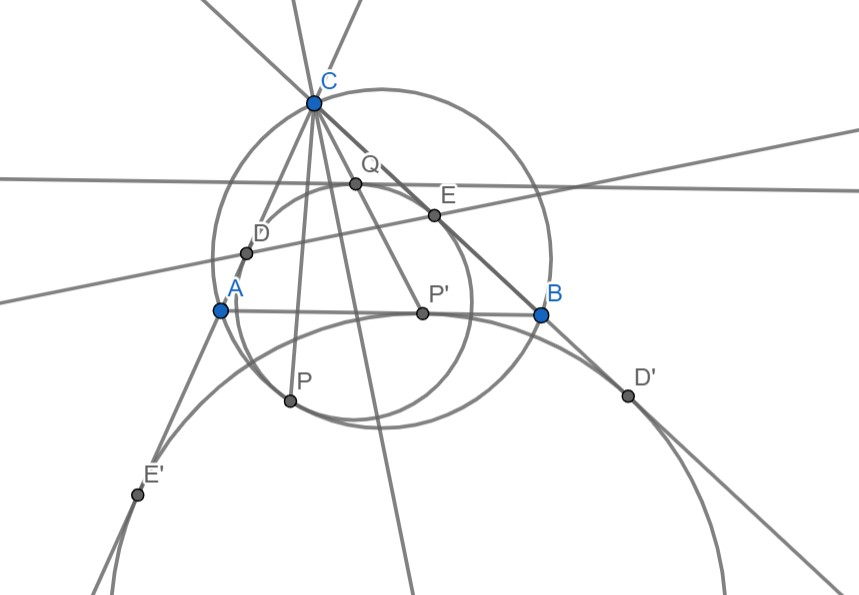
\includegraphics[scale=0.8]{egmo20135.jpg}
\end{center}
Wait, that's just the C-excircle. \newline
Amazing, so $P'$ is the excircle touch point. And $A$, $Q$, $P'$ are collinear by homothety. $\square$\newline
So yeah, whenever you spot mixtilinear incircles, excircles, or any symmetry about the angle bisector (e.g. AH and AO), try root bc inversion for the lolz.

\begin{problem} Let $D$, $E$, $F$ be the $A$-excircle contact points on $BC$, $AC$, $AB$ respectively. Let $\gamma$ be the circumcircle of $AEF$. Let $DE$ intersects $\Gamma$ again at $P$, and $DF$ intersects $\Gamma$ again at $Q$. Prove that $PQ$ is the A-midline. 
\end{problem}
\textbf{Solution:} Consider the inversion centered at $D$ taking $\Gamma$ to itself. In other words, it takes $E$ to $P$ and $F$ to $Q$. Since $BC$ is tangent to $(DEF)$, it must be parallel to $PQ$. Now we just need to prove $PQ$ passes through some nice midpoints. 

Consider the A-excenter, $X$. $X$ lies on $\Gamma$, so its image must be where $XD$ intersects $\Gamma$ again. Let's call that point $X'$. Since $AX$ is a diameter of $\Gamma$, $AX' \perp XD$. Since $XD \perp BC$, $AX' \parallel BC$. So $X'D$ is essentially the distance from $A$ to $BC$. We just need to prove that $PQ$ passes through its midpoint. This is clearly true, as the midpoint is the image of the antipode of $D$ on the excircle. $\square$\newline 

We used two OP techniques here. We applied an inversion with a negative power, and we mapped a circle onto itself. If you have read EGMO, you'd know that the second technique is related to orthogonal circles, because it often arises when the target is orthogonal to the reference circle. Obviously, orthogonal circles are nice, but even if they aren't there, you can just make up your own. \newline

Another example of negative inversion is the one sending the circumcircle to the nine-point circle. Understandably, a lot of points have really nice images, so when this technique is applicable, it's super powerful. It can completely cheese an IMO Q3.
\begin{problem}[IMO 2015/3] Let $ABC$ be an acute triangle with $AB>AC$. Let $\Gamma$ be its circumcircle, $H$ its orthocenter, and $F$ the foot of altitude from $A$. Let $M$ be the midpoint of $BC$. Let $Q$ be the point on $\Gamma$ such that $\angle HQA=90^{\circ}$ and let K be the point on $\Gamma$ such that $\angle HKQ=90^{\circ}$. Assume that $A$, $B$, $C$, $K$, $Q$ are all distinct and lie on $\Gamma$ in this order. Prove that the circumcircle of $KQH$ and $FKM$ are tangent to each other. 
\end{problem}
\begin{center}
    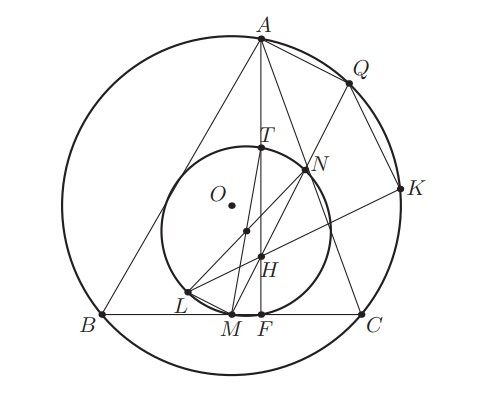
\includegraphics[scale=1]{figure836.jpg}
\end{center}
\textbf{Solution:} Immediately, we notice that $AF$ and $QM$ both pass through $H$. So it's natural to think of the inversion centred at H sending $A$ to $F$, $Q$ to $M$, and $K$ to $L$, where $L$ is a point on the nine-point circle. Notice that $\angle HML=90^{\circ}$, since inversion swapped the angles. This gives $LM \parallel AQ$. So to prove that $LM$ is tangent to $(AQL)$, we just need to prove $LA = LQ$. $KL$ intersects $\Gamma$ again at $Q^*$, the antipode of $Q$. So $AQ^* \perp AQ$. So $LT$ is the perpendicular bisector of $AQ$ by homothety at $H$. $\square$\newline
Note that this isn't the only orthocenter inversion. Orthocenter inversions are generally nice because the image of $ABC$ is similar to the orthic triangle of $ABC$. However, I've only used it once, so I'm probably not qualified to make further comments.

\section{Big Picture}
Sometimes a problem can seem pretty invertible, but contains a point whose image is absolutely horrendous. Take a look at the following problem:
\begin{problem}[ISL 2011/G4] Let $ABC$ be an acute triangle with circumcircle $\Omega$. Let $B_0$ be the midpoint of $AC$ and let $C_0$ be the midpoint of $AB$. Let $D$ be the foot of altitude from $A$, and let $G$ be the centroid of the triangle $ABC$. Let $\omega$ be a circle through $B_0$ and $C_0$ that is tangent to the circle $\Omega$ at a point $X \neq A$. Prove that the points $D$, $G$ and $X$ are collinear.
\end{problem}
\textbf{Solution:} Ewww, circle/circle tangencies. Wouldn't it be nice if $\Omega$ is a line? \newline
Inversion seems perfect for this question, since the images of $B$, $C$, $B_0$, $C_0$, and $D$ are all pretty nice. By extension, the image of $X$ should be nice too. However, you know what's not nice? $G'$.\newline
\begin{center}
    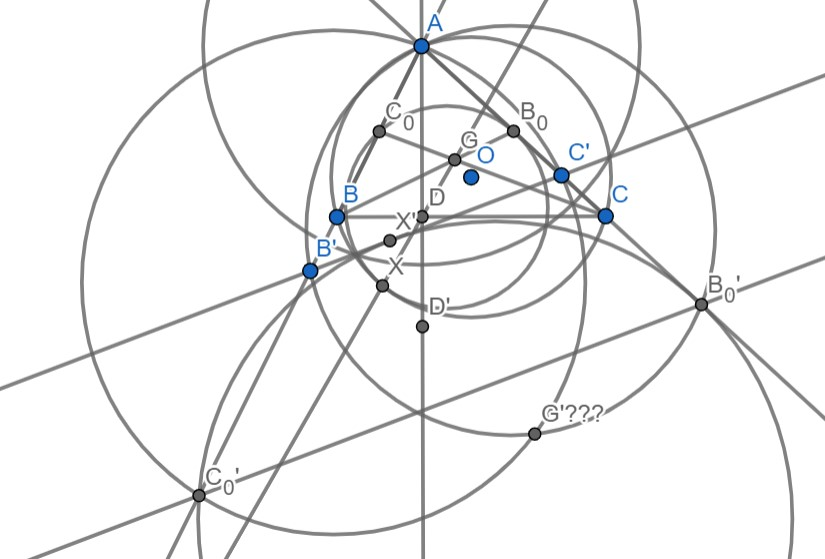
\includegraphics[scale=0.8]{isl2011g4r1.jpg} \\
    {\footnotesize Although any power would work for this question, I'm using $bc$. It's a nice habit to have because it leaves an extra tool at your disposal.}
\end{center}
Before we can invert, we need some setup. Specifically, we need to replace $G$ with a nicer point. A natural thought would be where $DG$ intersects $\Omega$ again, since $\Omega$ has a nice image. Let's label that point $E$. \newline
\begin{center}
    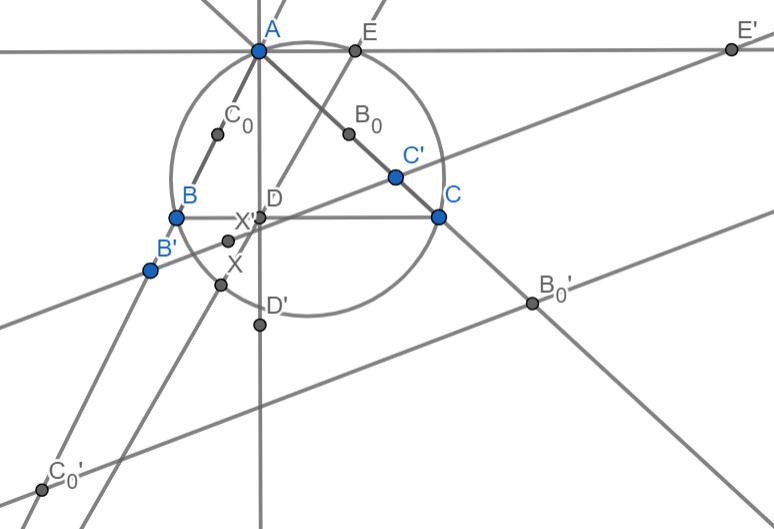
\includegraphics[scale=0.8]{isl2011g4r2.jpg}
\end{center}
If you stare at this diagram really hard, you might notice that $AE \parallel BC$! This is big, because now we don't even need $E'$. Since $\angle D'AE'=90^{\circ}$, if we can prove that $D'X' \perp B'C'$ then we are done! And it won't be long before you notice that $D'X'$ is the perpendicular bisector of $B_0'C_0'$. \newline 
The details are left as an exercise for the reader :) \newline 
Other times, inversion is used as a set-up for other techniques, most commonly complex bashing and projectives.
\begin{theorem}
The complex coordinate of a point $z$ inverted about the unit circle is $\cfrac{1}{\overline{z}}$
\end{theorem}
\begin{theorem}
Let $P'$ be the image of $P$ after inversion about the circle with diameter $AB$. Then $(A,B;P,P')=-1$. 
\end{theorem}
\begin{theorem}
Let $P'$ be the inverse of $P$. The polar of point $P$ (possibly at infinity) is the line passing through $P'$ perpendicular to $OP$.\newline
Notably, a point $X$ lies on the polar of a point $Y$ iff $Y$ lies on the polar of $X$. 
\end{theorem}
The last result is especially profound because it enables a new transformation --- pole-polar duality --- which turns points into lines and collinearity into concurrency. Unfortunately (fortunately?), as much as I'd like to go down this rabbit hole, we're going overtime. So I'll wrap up this handout with the famous Brocard's Theorem.
\begin{theorem}
Let $ABCD$ be a cyclic quadrilateral inscribed in circle $\omega$, and set $P=AB\cap CD$, $Q=BC\cap DA$, and $R=AC\cap BD$. Then $P$, $Q$, $R$ are the poles of $QR$, $RP$, $PQ$ with respect to $\omega$. 
\end{theorem}
\begin{center}
    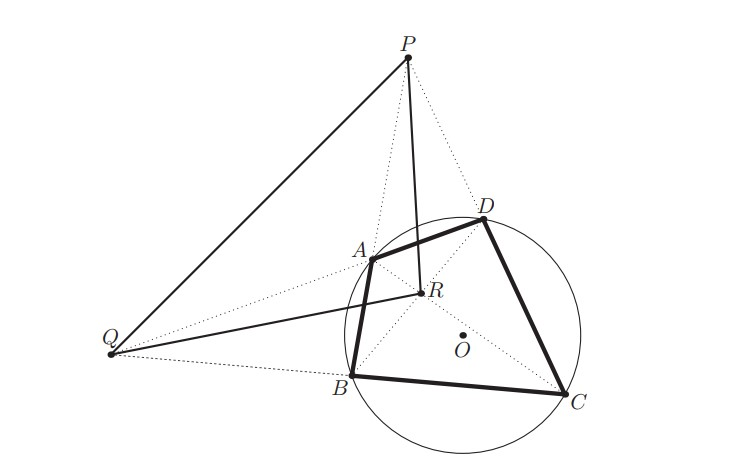
\includegraphics[scale=1]{figure95.jpg}
\end{center}
\end{document}